\chapter{Background Estimate} \label{chapter:background}

\section{Data-Driven Background Estimate}

    Selection does not remove all non-signal events.
    Indeed, most of the events remaining in the data are very likely background.
    Since these background events cannot be effectively differentiated from signal data,
        a technique must be used to estimate how much of the observed data is coming from background.
    Specifically, the analysis employs a method to predict the kinematic shape (in \mhh)
        of the background events within the 4b Signal Region,
        without directly observing that set of events.

    For the \vbfproc process, the background consists almost entirely of QCD jet events.
    The usual approach of simulating the background using Monte-Carlo techniques is not feasible,
        as such simulations are inaccurate when trying to model such complex, many-jet processes. [TODO: is this the actual reason?]
    Instead, the yield from background in the SR data is predicted based on the background yield in different subsets of the data.
        
    The fundamental assumption for this data-driven background estimate
        is that background events with only two b-tagged jets (2b data)
        will have kinematics very similar to the background events with 4 b-tagged (4b) jets.
    [TODO: double check what regions are used for what, since the 3b1f thing has made this weird]
    Thus, the kinematic distribution of the 2b signal region can be used as an estimate of the background in the 4b signal region.
    Unfortunately, the kinematics of the 2b and 4b data are not expected to match completely,
        so the 2b signal data must undergo a "reweighting" process,
        which adjusts the kinematic distribution to match that of 4b.
    This reweighting takes the form of a function $R$,
        which for each event $i$ takes a series of kinematic variables $x_i$ as an argument,
        and returns a reweighting value $r_i$ which scales that event's contribution to the kinematic distributions:
        $r_i = R(x_i)$.
    Deriving this function, and determining the appropriate inputs for it,
        are the challenges addressed in the following sections.

\section{Neural Network Training and Uncertainty} \label{sec:nn_training}

    The reweighting function is derived using machine learning techniques.
    A neural network (NN) is trained to identify how to reweight 2b data such that the cumalitive kinematic distribution looks like that of 4b data.
    In order to improve stability in the reweighting function,
        an ensemble of 100 networks is trained, and the median of their calculations is used (called the ``Nominal Estimate'').
    Each neural network instance $j$ produces a reweighting factor $w_{ij}$, and has a normalization factor $\alpha_j$ associated with it.
    This normalization factor is calculated so the total yield of all 2b reweighted events matches that of the 4b yield in the same region. 
    % TODO: I need to emphasize that the normalization is set to match the yield of
    % the region the NN was *trained* in. 
    % So in going from 2b CR to 4b CR, there is some scaling factor "a"
    % That same "a" is then applied when going from 2b SR to 4b SR
    % Key point being that we are not artificially forcing the 
    % 4b SR background yield to match the 4b SR data yield.
    So for $N$ total 2b events and $N'$ total 4b events:
        \begin{equation}
        \sum_{i=1}^{N} \alpha_j w_{ij} = N'
        \end{equation}

    The nominal estimate $\tilde{w}$ constructed from the median of these networks will not necessarily satisfy this same relation,
        so it is given its own separate normalization $\tilde \alpha$:
        \begin{equation}
        \sum_{i=1}^{N} \tilde \alpha \tilde w_i = N'
        \end{equation}

    \begin{figure}[!htbp]
        \subfloat[Data before reweighting]{
            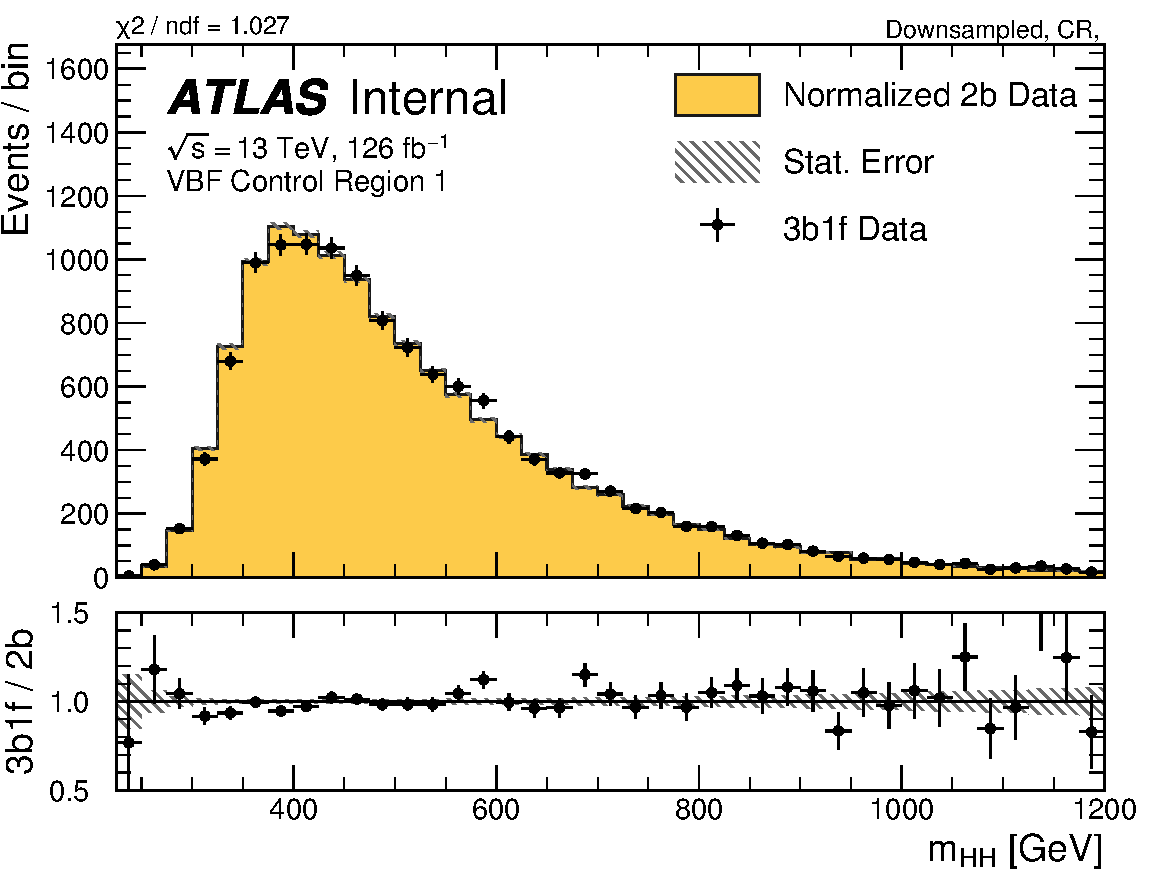
\includegraphics[width=0.5\linewidth,height=\textheight,keepaspectratio]{background/NR-MAY21-crypto-m_hh-control-no_rw-allyr-3b1f-dEtahhcat_inclusive}
        }
        \subfloat[Data after reweighting]{
            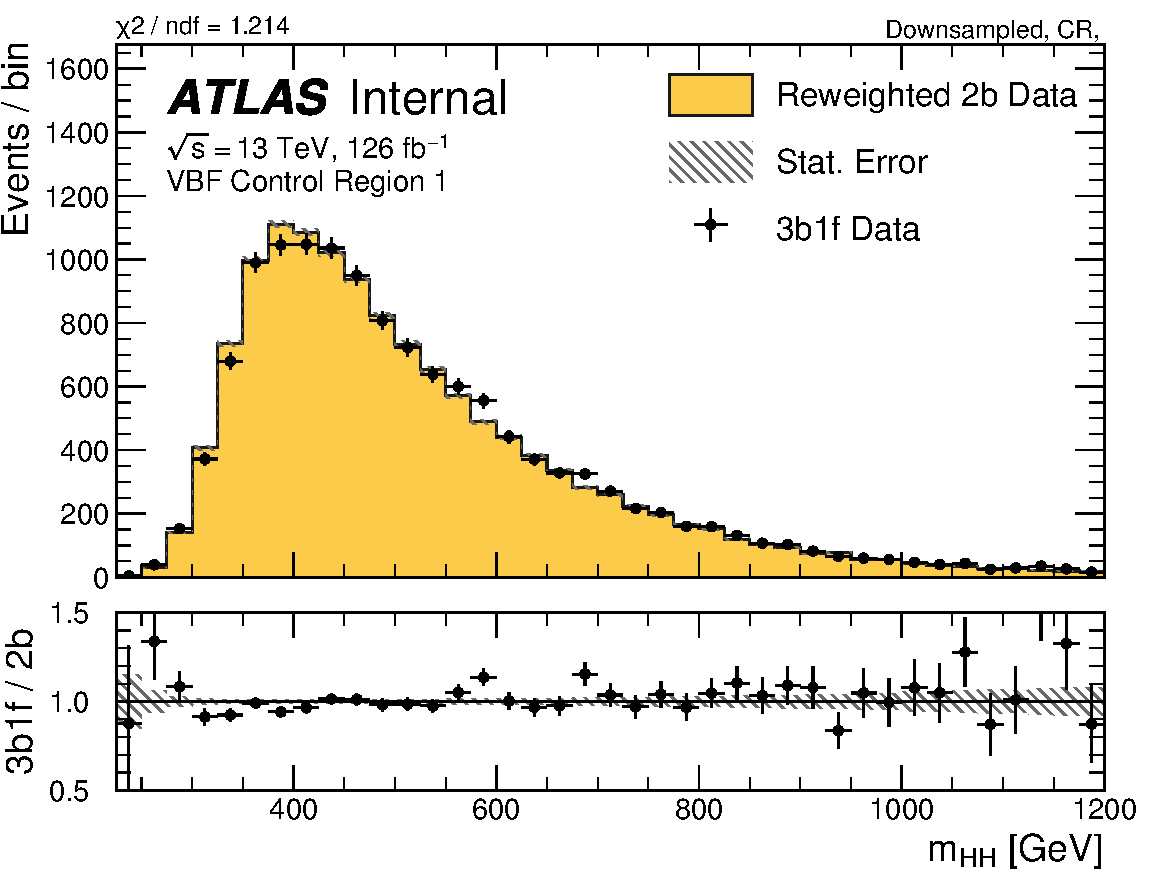
\includegraphics[width=0.5\linewidth,height=\textheight,keepaspectratio]{background/NR-MAY21-crypto-m_hh-control-NN-allyr-3b1f-dEtahhcat_inclusive}
        }
        \caption{
            The \mhh kinematic distribution of the 2b VS 4b regions, before and after reweighting the 2b region.
            [TODO: these look ... very similar. Am I using the right plots?]
        }
        \label{fig:data_mhh_reweight}
    \end{figure}

    The problem with this training approach, is that the 4b signal region cannot be used in the training.
    Instead, the neural networks are trained using the Control Region data,
        and are optimized to reweight the 2b CR data to resemble the 4b CR data.
    Because the reweighting function is trained on a different kinematic region than the signal region,
        a systematic uncertainty is associated with it.
    This is calculated by training a different ensemble of NNs on yet another kinematic region (Validation).
    % TODO you need to elaborate on the quandrant Signal scheme in order to describe
    % precisely how the error is calculated
    The difference between the median of these validation-trained NNs and the nominal estimate
        produces a ``shape uncertainty'' for the reweighting.
    The shape uncertainty is symmetrized around the nominal estimate to produce the final systematic uncertainty
        associated with the reweighting procedure.
    A comprehensive error for the background estimate is produced by combing the shape uncertainty with the statistical error
        associated with the limited sample size of the training data.


\section{VBF Background Reweighting Variables} \label{sec:vbf_bgdNNRW}

    The Neural Network used to reweight the 2b-Tagged Control-Region data into the 4b Signal region
        uses a different set of variables when trained for the VBF process than it does for ggF.
    This list of variables was selected through two correlation tests,
        the first of which was determining how strongly correlated different variables are to \mhh
        (Figure \ref{fig:mhh_corr}).

    \begin{figure}[!htbp]
        \subfloat[$\deta \leq 1.5$]{
            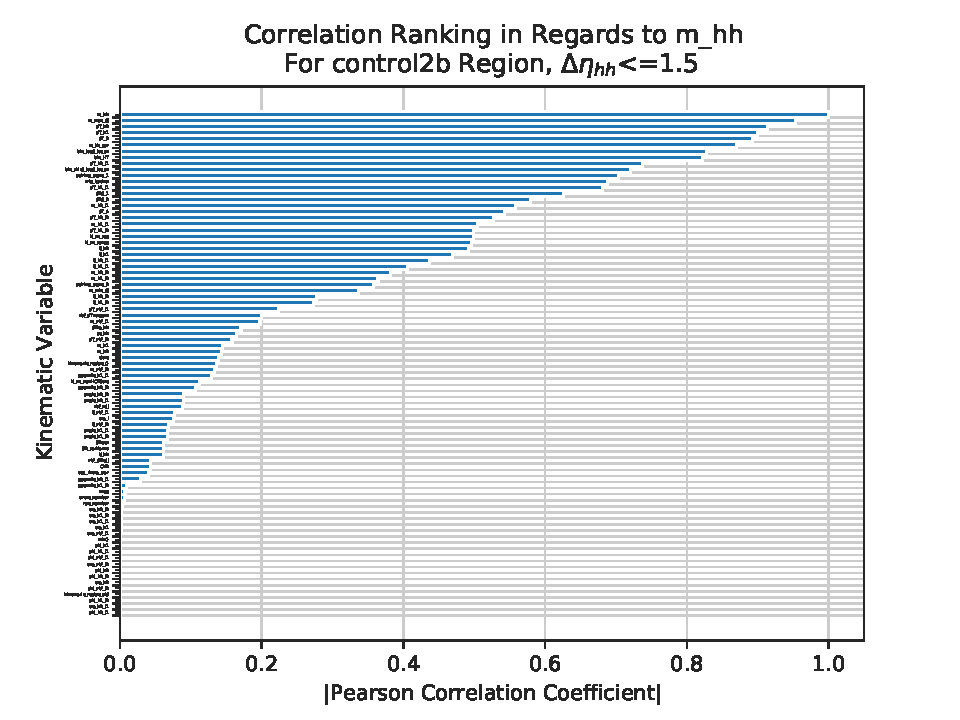
\includegraphics[width=0.5\linewidth,height=\textheight,keepaspectratio]{background/correlation_control2b_detahh-LTE1p5_hist_m_hh.pdf}
        }
        \subfloat[$\deta > 1.5$]{
            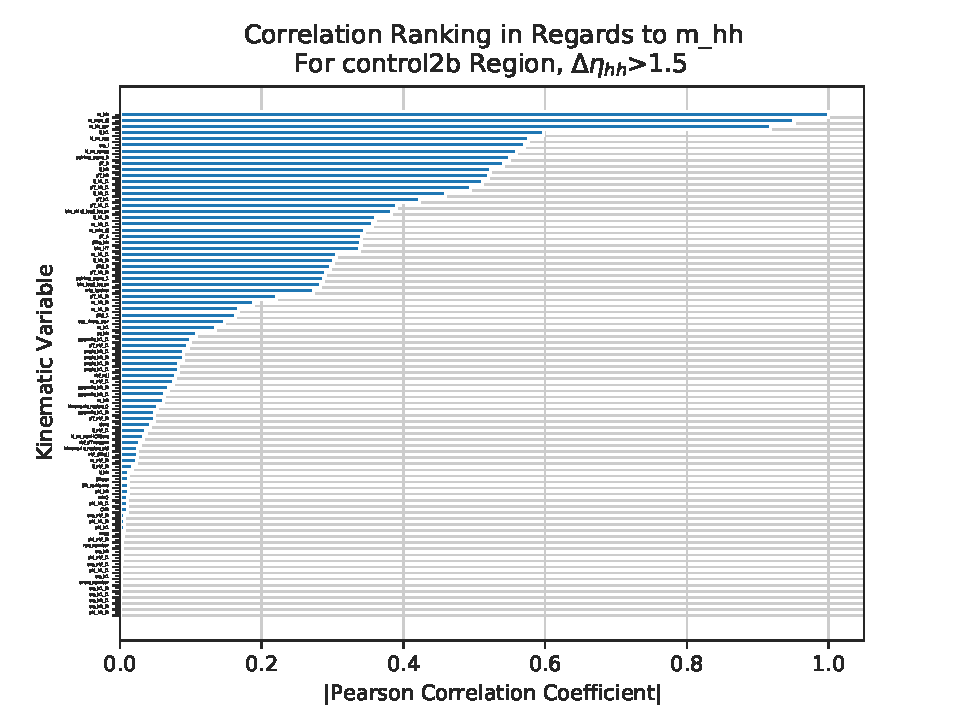
\includegraphics[width=0.5\linewidth,height=\textheight,keepaspectratio]{background/correlation_control2b_detahh-GT1p5_hist_m_hh.pdf}
        }
        \caption{
            The Pearson Correlation Coefficients associated with \mhh for the 2b Control Region data.
            The regions in which $\deta \leq 1.5$ and $\deta>1.5$ are separately displayed.
            The higher up on the chart a variable is, the more strongly correlated it is to \mhh,
                with \mhh itself at the top with a coefficient of 1.
            Note that most of the VBF-specific variables, such as vbf\_mjj, are very poorly correlated to \mhh and thus not proffered.
        }
        \label{fig:mhh_corr}
    \end{figure}

    Based on their high correlation to \mhh in both \deta regions, 23 variables were then selected for further study.
    These 23 variables were plotted against each other in a correlation matrix,
        which displayed how strongly correlated these variables are to each other.
    A final set of seven variables was selected based (Table \ref{tab:vbf_NNRW_vars}) on which variables were \textit{least} correlated to each other,
        in order to avoid variables carrying redundant information (Figure \ref{fig:vbf_corr_matrix}).

    \begin{figure}[!htbp]
        \subfloat[$\deta \leq 1.5$]{
            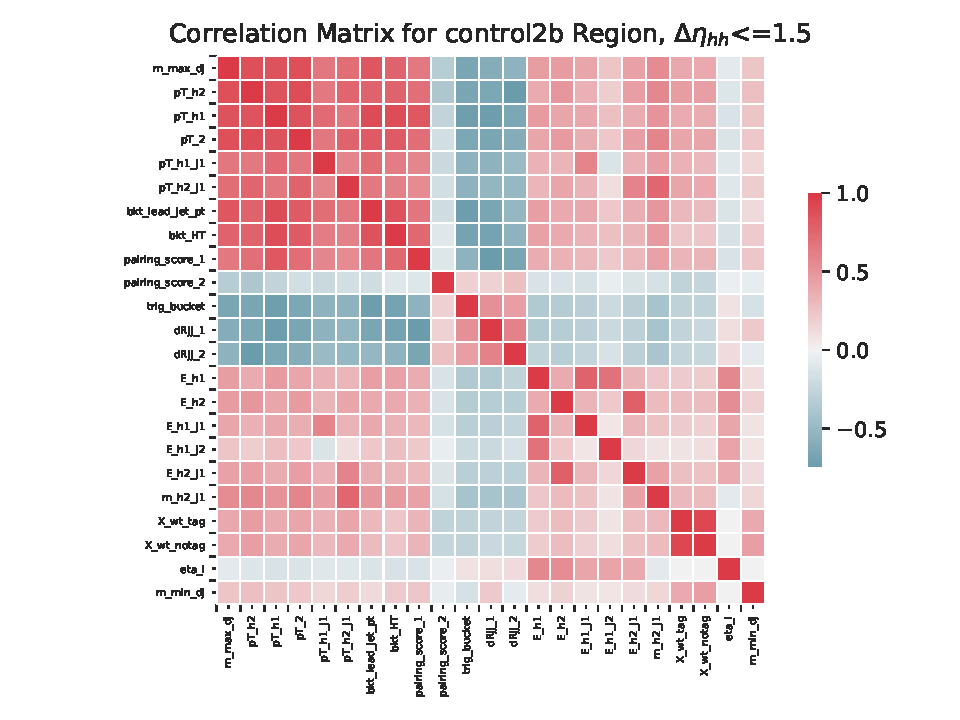
\includegraphics[width=0.5\linewidth,height=\textheight,keepaspectratio]{background/correlation_control2b_detahh-LTE1p5_matrix.pdf}
        }
        \subfloat[$\deta > 1.5$]{
            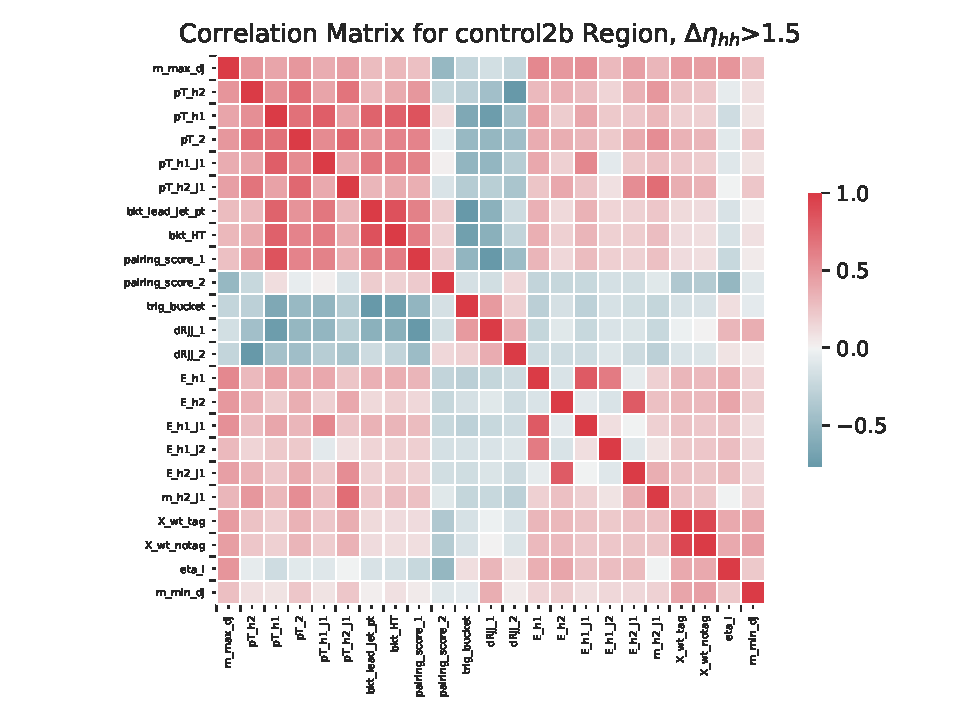
\includegraphics[width=0.5\linewidth,height=\textheight,keepaspectratio]{background/correlation_control2b_detahh-GT1p5_matrix.pdf}
        }
        \caption{
            The Pearson Correlation Coefficients matrix associated with variables in the 2b Control Region data.
            The regions in which $\deta \leq 1.5$ and $\deta>1.5$ are separately displayed.
            Bins with more saturated (i.e.\ more blue or more red) colors indicate strong correlation between those two variables.
            All variables are of course 100\% correlated to themselves, hence the deep red line running down the diagonal.
            The most highly preferred variables are those with correlation coefficients near 0 for as many other variables as possible.
            If a variable (i.e.\ m\_max\_dj) is selected, any other variables with strong correlations to it (i.e.\ pT\_h2)
                are then strongly disfavored for later selection.
        }
        \label{fig:vbf_corr_matrix}
    \end{figure}


    \begin{table}[!htbp] \centering \footnotesize
    \caption{Final Set of Neural Network Variables}
    \label{tab:vbf_NNRW_vars}
    \begin{tabular}{ |l|l|l| }
        \hline
        \textbf {Variable} & \textbf {Internal Name} & \textbf {Description} \\
        \hline
        $M_{max \Delta j}$ & \code{m\_max\_dj}         & 
            Take the di-jet mass of the six possible pairings\\
            && of the four higgs’ candidate jets;\\
            && this is the maximum di-jet mass of those pairings \\ 
        \hline
        $M_{min \Delta j}$ & \code{m\_min\_dj}         & 
            As above, but the minimum \\
        \hline
        $E_{H1}$           & \code{E\_h1}              & 
            Energy of the leading-$p_T$ reconstructed Higgs \\
        \hline
        $E_{H2}$           & \code{E\_h2}              & 
            Energy of the sub-leading-$p_T$ reconstructed Higgs \\
        \hline
        Xwt-tag            & \code{X\_wt\_tag}         & 
            $\log\left(X_{Wt}\right)$, where $X_{Wt}$ is the variable used for the top veto \\
        \hline
        $\eta_i$           & \code{eta\_i}             & 
            Average $\eta$ of the four Higgs decay jets \\
        \hline
        Pairing Score 2    & \code{pairing\_score\_2 } & 
            This changes depending on the Higgs pairing algorithm used. \\
            &&The current algorithm used is minDR. \\
            &&With four jets, there are three possible pairings of the jets. \\
            &&The pairings are ranked by the $\Delta_R$ of the leading-$p_T$ Higgs candidate. \\
            &&Pairing Score 2 is the $\Delta-R$ of the second-smallest of these pairings. \\
        \hline
    \end{tabular} \end{table}



\section{Statistical Error}

    TODO: I don't even want to bother with this until the group figures out what to do.
%
%    Now to talk about statistical error in the Neural network estimate
%
%    Poisson stat errors: stat error on bin i is 
%        \begin{equation}
%        \sigma_i = \sqrt{\sum_{j \in i} w_j^2}
%        \end{equation}
%
%    Bootstrap uncertainty: A bin-by-bin statistical error resulting from the variations in each of the networks' reweighting functions.
%    Naively, this would mean using the average of all networks, with an error calculated as the standard deviation of all histograms of all the networks, for a given variable of interest.
%    Slightly less naively (to make us more robust to outliers),
%        we would use the median of all networks, and the IQR values of the networks as the error.
%    In reality, it's impractical to retain the information of all networks for all histograms.
%    We can still use the median value, but the error has to be calculated another way.
%    Specifically, the error is calculated by storing a small amount of extra information regarding the IQR of the bootstraps.
%    Whenever a kinematic distribution is produced, \textbf{two} histograms are generated:
%        the nominal histogram, and the \textit{varied} histogram.
%    The difference between the values of the nominal and varied histograms, per bin,
%        are taken as the error on that bin for the nominal histogram.
%
%    The nominal event weights are calculated as
%        \begin{equation}
%        \tilde w_i = \textrm{median}(\alpha_1 w_{1,i}, ..., \alpha_{100} w_{100,i})
%        \end{equation}
%        with the normalization $\tilde \alpha$ calculated as described above.
%    So if the yield of normalized nominal weights is denoted
%        \begin{equation}
%        \tilde Y \equiv \sum_{i=1}^{N} \tilde \alpha \tilde w_i = \textrm{yield of 4b control region}
%        \end{equation}
%    then the values of the bins of the nominal histogram, $H_j$ are:
%        \begin{equation}
%        H_j = \tilde \alpha \sum_{i \in j} \tilde w_i
%        \end{equation}
%
%    A "weight variation" factor is calculated per event as 
%        \begin{equation}
%        V^w_i = \frac{1}{2}\textrm{IQR}(w_{1,i}, w_{2,i}, ..., w_{100,i})
%        \end{equation}
%    Likewise, a "normalization variation" factor is calculated as
%        \begin{equation}
%        V^{\alpha} = \frac{1}{2}\textrm{IQR}(\alpha_{1}, \alpha_{2}, ..., \alpha_{100})
%        \end{equation}
%    The sum of the varied weights is 
%        \begin{equation}
%        Y_v = \sum_{i=1}^{N} \left( \tilde w_i + V^w_i \right)
%        \end{equation}
%    And the ratio of the nominal yield to the varied yield is $R_Y \equiv \tilde Y / Y_v$
%
%    The "varied" histogram $H'$ is then calculated based on these variation factors as:
%        \begin{equation} \begin{split}
%        H'_j &= \left[ R_Y \sum_{i \in j} \tilde w_i + V^w_i \right] + V^{\alpha} H_j
%        \\H'_j &= \sum_{i \in j} \left[ R_Y \left( \tilde w_i + V^w_i \right)
%            + V^{\alpha} \tilde \alpha \tilde w_i \right]
%        \end{split} \end{equation}
%
%    The error of the nominal histogram bin $j$ then is
%        \begin{equation} \begin{split}
%        \sigma_j &= | H'_j - H_j |
%        \\&= \left| \sum_{i \in j} \left[
%            R_Y \left( \tilde w_i + V^w_i \right)
%            + V^{\alpha} \tilde \alpha \tilde w_i \right] 
%            -\tilde \alpha \sum_{i \in j} \tilde w_i \right|
%        \\&= \left| \sum_{i \in j} \left[
%            R_Y \left( \tilde w_i + V^w_i \right)
%            + V^{\alpha} \tilde \alpha \tilde w_i 
%            - \tilde \alpha \tilde w_i
%            \right] \right|
%        \\&= \left| \sum_{i \in j} \left[
%            R_Y \left( \tilde w_i + V^w_i \right) 
%            + \tilde \alpha \tilde w_i (V^{\alpha}-1) \right] \right|
%        \end{split} \end{equation}
%
